\documentclass[12pt,a4paper]{article}

\usepackage{xeCJK}
\usepackage{amsmath,amsthm,amssymb}
\usepackage[colorlinks,linkcolor=blue]{hyperref}
\usepackage{graphicx}
\usepackage{tikz}
\usepackage{xcolor}
\usepackage{float}
\usepackage{makeidx}
\usepackage{listings} 
\usepackage[]{caption2}
\usepackage[numbers,sort&compress]{natbib}
\usepackage[level]{datetime}
\usepackage{indentfirst}
\usepackage{enumitem}
%\usepackage{draftwatermark}
\usepackage{titlesec}
\usepackage{fancyhdr}
\usepackage[top=1.5cm, bottom=2cm, outer=1.5cm, inner=1.5cm, heightrounded, marginparwidth=0cm, marginparsep=0cm]{geometry}
%\usepackage{showframe}

\renewcommand{\today}{\number\year 年 \number\month 月 \number\day 日}
\renewcommand{\refname}{参考文献}
\renewcommand{\tablename}{表}
\renewcommand{\figurename}{图}
\renewcommand{\captionlabeldelim}{}
\renewcommand{\contentsname}{目录}

\newcommand{\upcite}[1]{\textsuperscript{\textsuperscript{\cite{#1}}}}
\newcommand{\tabincell}[2]{\begin{tabular}{@{}#1@{}}#2\end{tabular}}

\definecolor{dkgreen}{rgb}{0,0.6,0}
\definecolor{gray}{rgb}{0.5,0.5,0.5}
\definecolor{mauve}{rgb}{0.58,0,0.82}
\lstset{
  language=c++, 
  basicstyle=\footnotesize,  
  % numbers=left,      
  numberstyle=\tiny\color{gray}, 
  stepnumber=2, 
  numbersep=5pt,
  backgroundcolor={},
  showspaces=false,   
  showstringspaces=false,
  showtabs=false,         
  frame=single,                   % frame around code [single, shadowbox]
  rulecolor=\color{black}, 
  tabsize=2,                     
  captionpos=b,                   % caption-position bottom
  breaklines=true,                % automatic line breaking
  breakatwhitespace=false, 
  % title=\lstname,               % filename included with \lstinputlisting;
  keywordstyle=\color{blue},     
  commentstyle=\color{dkgreen}, 
  stringstyle=\color{mauve},     
  escapeinside={\%*}{*)},         % if want to add LaTeX within your code
  morekeywords={*,...}            % if want to add more keywords to the set
}

%\SetWatermarkText{\textsc{CGGOS}}
%\SetWatermarkScale{1}
%\SetWatermarkFontSize{4cm}
%\SetWatermarkLightness{0.5}

%\newpagestyle{main}{            
%  \sethead{}{VINS-Mono 论文公式推导与代码解析}{\url{https://cggos.github.io}}
%  \headrule
%  \setfoot{}{}{}
%%  \footrule
%}
%\pagestyle{main} 

\pagestyle{fancy}
\lhead{}
\chead{S-MSCKF论文公式推导与代码解析}
\rhead{}
\lfoot{更新于 \date{\today}}
\cfoot{\thepage}
\rfoot{\url{https://github.com/cggos}}
\renewcommand{\headrulewidth}{0.4pt}
\renewcommand{\footrulewidth}{0.4pt}

\bibliographystyle{unsrt}

\title{S-MSCKF论文公式推导与代码解析}
\author{高洪臣}
\date{2019年9月1日}


\begin{document}

\maketitle
\tableofcontents

\noindent
\setlength{\parindent}{2em}
\setlength{\parskip}{0.3em}
\linespread{1}

\newpage
\section{概述}

\subsection{MSCKF}

MSCKF全称Multi-State Constraint Kalman Filter(多状态约束下的Kalman滤波器),是一种基于滤波的VIO算法,2007年由明尼苏达州大学Mourikis在~\cite{mourikis2007multi}中首次提出。MSCKF在EKF框架下融合IMU和视觉信息,相较于单纯的VO算法,MSCKF能够适应更剧烈的运动、一定时间的纹理缺失等,具有更高的鲁棒性;相较于基于优化的VIO算法(VINS,OKVIS),MSCKF精度相当,速度更快,适合在计算资源有限的嵌入式平台运行。在机器人、无人机、AR/VR领域,MSCKF都有较为广泛的运用,如Google Project Tango就用了MSCKF进行位姿估计。

\subsection{MSCKF vs EKF-SLAM}

在传统的EKF-SLAM框架中,特征点的信息会加入到特征向量和协方差矩阵里,这种方法的缺点是特征点的信息会给一个初始深度和初始协方差,如果不正确的话,极容易导致后面不收敛,出现inconsistent的情况。MSCKF维护一个pose的FIFO,按照时间顺序排列,可以称为滑动窗口,一个特征点在滑动窗口的几个位姿都被观察到的话,就会在这几个位姿间建立约束,从而进行KF的更新。~\cite{xinliang-zhong-msckf_notes}

\begin{figure}[!htbp]
\centering
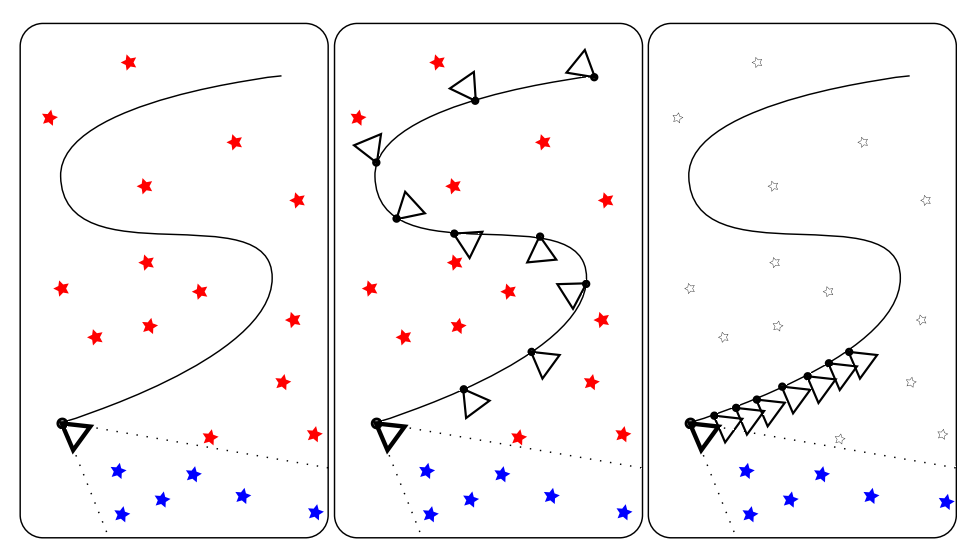
\includegraphics[scale=0.25]{images/ekf-slam-vs-msckf.png}
\caption{EKF-SLAM, keyframe-based SLAM, MSCKF}
\end{figure}

\subsection{S-MSCKF}

S-MSCKF~\cite{sun2018robust}是宾夕法尼亚大学Vijay Kumar实验室开源的双目版本MSCKF算法。

% 代码(注释版): \href{https://github.com/cggos/msckf_vio_cg}{cggos/msckf\_vio\_cg} 

\begin{figure}[!htbp]
\centering
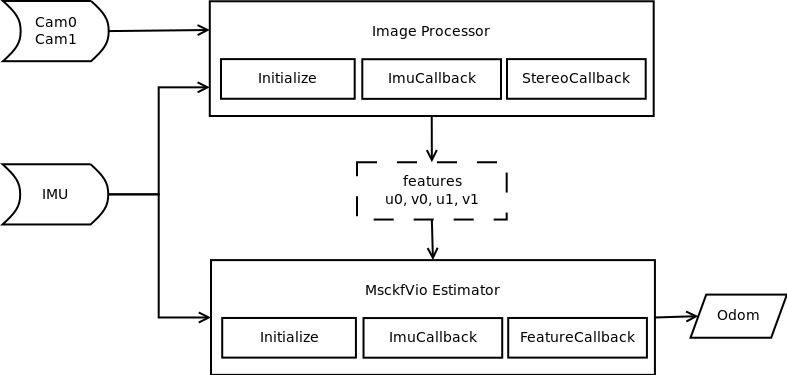
\includegraphics[scale=0.5]{images/msckf_vio_io.png}
\end{figure}

\newpage
\section{Image Processor}

\subsection{代码流程}

\subsubsection{Initialize}

\begin{itemize}
\item load parameters
\item create \verb|FastFeatureDetector|
\end{itemize}

\subsubsection{ImuCallback}

第一帧图像后,不断添加IMU message到 \verb|imu_msg_buffer|。

\subsubsection{StereoCallback}

\begin{figure}[!htbp]
\centering
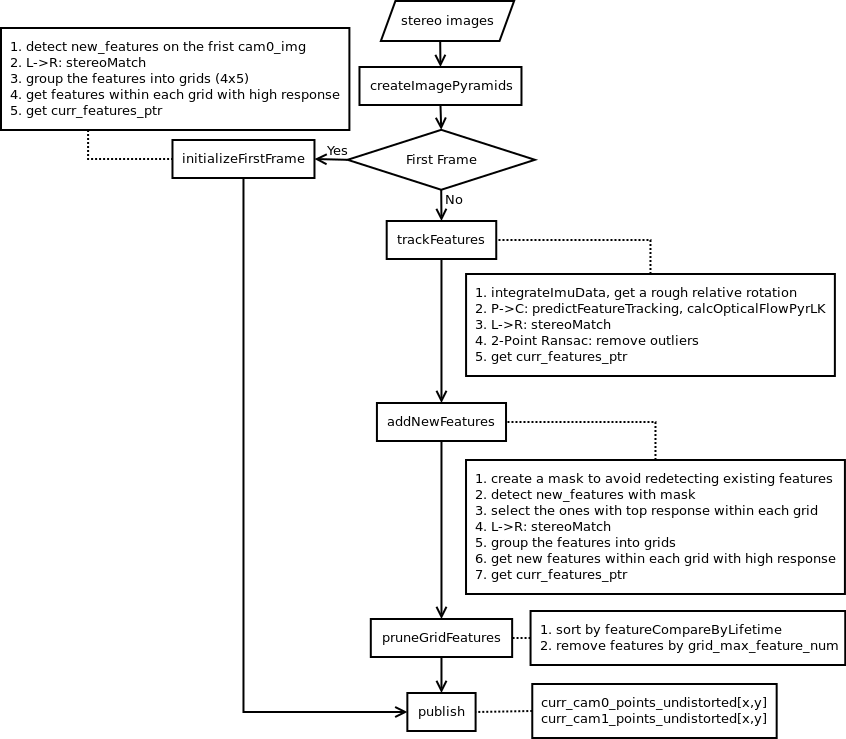
\includegraphics[scale=0.6]{images/stereo_cb.png}
\caption{StereoCallback流程图}
\end{figure}


\newpage
\section{MsckfVio Estimator/Filter}

\subsection{Overview}

\subsubsection{Kalman Filter}

\begin{figure}[!htbp]
\centering
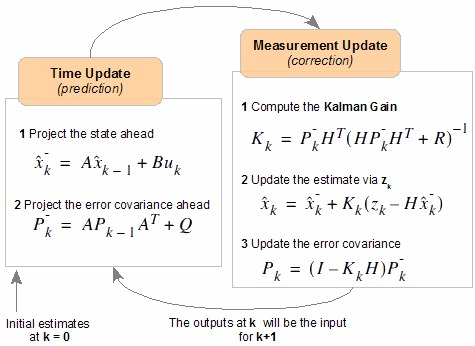
\includegraphics[scale=0.7]{images/kf_flow.jpg}
\caption{Kalman Filter流程图}
\end{figure}

\subsubsection{Multi-State Constraint Filter}

\begin{figure}[!htbp]
\centering
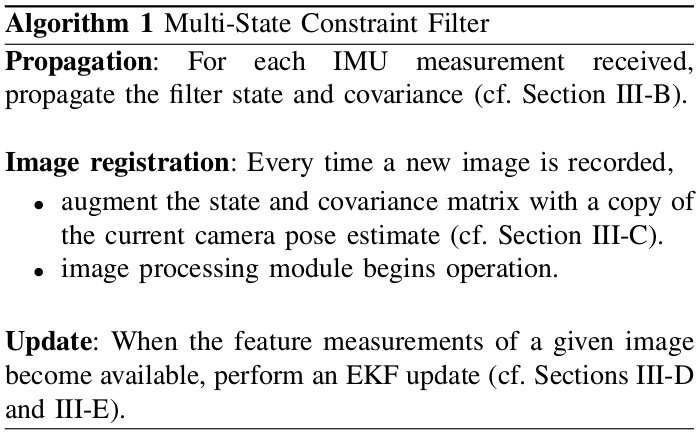
\includegraphics[scale=0.6]{images/msckf_algr.png}
\caption{Multi-State Constraint Filter 流程图}
\end{figure}

\subsection{代码流程}

\subsubsection{Initialize}

\begin{itemize}
\item Load Parameters
\item Initialize state server: \verb|state_server.continuous_noise_cov|
\item Initialize the \textbf{chi squared test table} with confidence level \textbf{P=0.95} for \verb|MsckfVio::gatingTest()|
\begin{lstlisting}
for (int i = 1; i < 100; ++i) {
    boost::math::chi_squared chi_squared_dist(i);
    chi_squared_test_table[i] = boost::math::quantile(chi_squared_dist, 0.05);
}
\end{lstlisting}
\begin{figure}[!htbp]
\centering
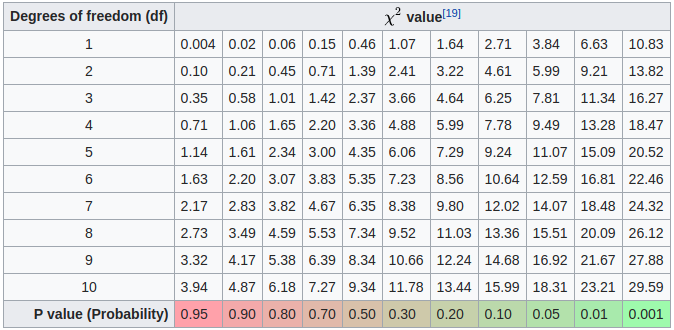
\includegraphics[scale=0.6]{images/chi_square_table.png}
\caption{chi-square table}
\end{figure}
\end{itemize}

\subsubsection{ImuCallback}

\begin{itemize}

\item 添加IMU message到 \verb|imu_msg_buffer|

\item \verb|initializeGravityAndBias|,要求前200帧IMU静止不动

\begin{itemize}
\item 将前200帧加速度和角速度求平均
\item 平均角速度作为陀螺仪的bias: \verb|state_server.imu_state.gyro_bias|
\item 平均加速度作为IMU系下的重力加速度:\verb|gravity_imu|
\item 平均加速度的模值作为重力加速度模长g:\verb|IMUState::gravity|
\item 计算初始时刻World系(水平天向)重力向量(0,0,-g)和IMU系重力向量\verb|gravity_imu|之间的姿态(旋转四元数):\verb|state_server.imu_state.orientation|
\end{itemize}

\end{itemize}

\subsubsection{FeatureCallback}

\begin{figure}[!htbp]
\centering
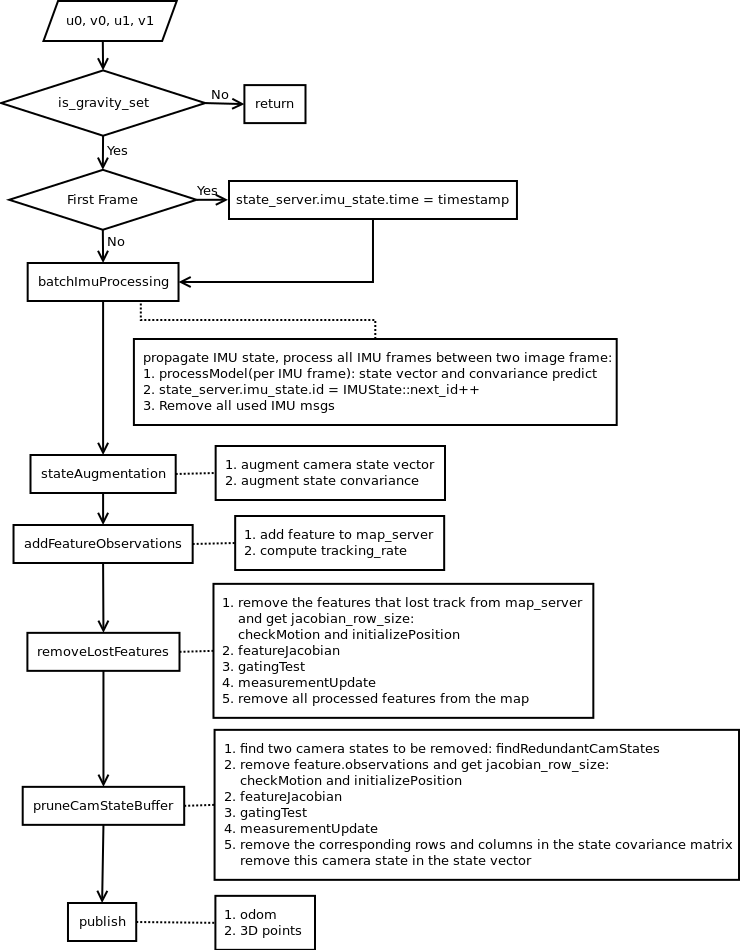
\includegraphics[scale=0.7]{images/feature_cb.png}
\caption{FeatureCallback流程图}
\end{figure}

\newpage
\subsection{EKF状态向量}

IMU状态向量(true-state)

\begin{equation*}
\mathbf{x}_{I} = 
\left(
{}^I_G \mathbf{q}^\top \quad 
\mathbf{b}_g^\top \quad 
{}^G\mathbf{v}^\top_I \quad 
\mathbf{b}_a^\top \quad
{}^G\mathbf{p}^\top_I \quad
{\color{blue}
{}^I_C \mathbf{q}^\top \quad
{}^I\mathbf{p}^\top_C}
\right)^\top
\in \mathbb{R}^{22 \times 1}
\end{equation*}

IMU误差状态向量

\begin{equation*}
\tilde{\mathbf{x}}_{I} = 
\left(
{}^I_G \tilde{\boldsymbol{\theta}}^\top \quad 
\tilde{\mathbf{b}}_g^\top \quad 
{}^G\tilde{\mathbf{v}}^\top_I \quad 
\tilde{\mathbf{b}}_a^\top \quad
{}^G\tilde{\mathbf{p}}^\top_I \quad
{\color{blue}
{}^I_C \tilde{\boldsymbol{\theta}}^\top \quad
{}^I\tilde{\mathbf{p}}^\top_C}
\right)^\top 
\in \mathbb{R}^{21 \times 1}
\end{equation*}

IMU噪声向量

\begin{equation*}
\mathbf{n}_I^\top = 
\left(\mathbf{n}_g^\top \; \mathbf{n}_{wg}^\top \; \mathbf{n}_a^\top \; \mathbf{n}_{wa}^\top\right)^\top
\in \mathbb{R}^{12 \times 1}
\end{equation*}

其对应的噪声协方差矩阵

\begin{equation*}
\mathbf{Q}_I 
= \mathbb{E}\left[\mathbf{n}_I^{}\mathbf{n}_I^\top\right]
= \text{diag}\left( 
\sigma_{g}^2  \mathbf{I}_{3\times3 } \quad
\sigma_{bg}^2 \mathbf{I}_{3\times3 } \quad
\sigma_{a}^2  \mathbf{I}_{3\times3 } \quad
\sigma_{ba}^2 \mathbf{I}_{3\times3 } 
\right)
\in \mathbb{R}^{12 \times 12}
\end{equation*}

Camera误差状态向量

\begin{equation*}
\tilde{\mathbf{x}}_{C_i} = 
\left(
{}^{C_i}_G\tilde{\boldsymbol{\theta}}^\top \quad
{}^G\tilde{\mathbf{p}}_{C_i}^\top
\right)^\top
\in \mathbb{R}^{6 \times 1}
\end{equation*}

系统(Imu+Camera)误差状态向量

\begin{equation*}
\tilde{\mathbf{x}} = 
\left(
\tilde{\mathbf{x}}_I^\top \quad
\tilde{\mathbf{x}}_{C_1}^\top \quad
\cdots \quad 
\tilde{\mathbf{x}}_{C_N}^\top
\right)^\top
\in \mathbb{R}^{(21+6N) \times 1}
\end{equation*}


\subsection{Propagation/Prediction}

\subsubsection{IMU误差状态方程}

IMU运动微分方程(nominal-state状态方程)

\begin{equation}
\label{equ:imu_diff_func_nominal_state}
\hat{\mathbf{x}} = 
\begin{cases}
\begin{aligned}
{}^I_G\dot{\hat{\mathbf{q}}} &= \frac{1}{2}\Omega(\hat{\boldsymbol{\omega}}) {}^I_G\hat{\mathbf{q}} \\
\dot{\hat{\mathbf{b}}}_g &= \mathbf{0}_{3\times 1} \\
{}^G\dot{\hat{\mathbf{v}}} &= C\left({}^I_G\hat{\mathbf{q}}\right)^\top \hat{\mathbf{a}} + {}^G\mathbf{g} \\
\dot{\hat{b}}_a &= \mathbf{0}_{3\times 1}, \\
{}^G\dot{\hat{\mathbf{p}}}_I &= {}^G\hat{\mathbf{v}} \\
{}^I_C\dot{\hat{\mathbf{q}}} &= \mathbf{0}_{3\times 1} \\
{}^I\dot{\hat{\mathbf{p}}}_C &= \mathbf{0}_{3\times 1}
\end{aligned}
\end{cases}
\end{equation}

其中,

\begin{equation*}
\begin{aligned}
\hat{\boldsymbol{\omega}} = \boldsymbol{\omega}_m - \hat{\mathbf{b}}_g, \quad
\hat{\mathbf{a}} = \mathbf{a}_m - \hat{\mathbf{b}}_a
\end{aligned}
\end{equation*}

并且(使用JPL四元数)

\begin{equation*}
\Omega\left(\hat{\boldsymbol{\omega}}\right) 
\triangleq 
{\begin{bmatrix}
\hat{\boldsymbol{\omega}} \\ 0
\end{bmatrix}}_R
= 
\begin{pmatrix}
-[\hat{\boldsymbol{\omega}}_\times] & \boldsymbol{\omega} \\
-\boldsymbol{\omega}^\top & 0
\end{pmatrix}
\end{equation*}

根据 \cite{DBLP:journals/corr/abs-1711-02508} ESKF 中 \textit{\textbf{5.3.3 The error-state kinematics}} 小节公式,IMU error-state状态方程

\begin{equation}
\label{equ:imu_diff_func_error_state}
\dot{\delta \mathbf{x}}_{I} = 
\begin{cases}
\begin{aligned}
\dot{\delta \mathbf{p}} &= \delta \mathbf{v} \\
\dot{\delta \mathbf{v}} &= -\mathbf{R}\left[\mathbf{a}_{m}-\mathbf{a}_{b}\right]_{ \times} \delta \boldsymbol{\theta}-\mathbf{R} \delta \mathbf{a}_{b}+\delta \mathbf{g}-\mathbf{R} \mathbf{a}_{n} \\
\dot{\delta \boldsymbol{\theta}} &= -\left[\boldsymbol{\omega}_{m}-\boldsymbol{\omega}_{b}\right]_{ \times} \delta \boldsymbol{\theta}-\delta \boldsymbol{\omega}_{b}-\boldsymbol{\omega}_{n} \\
\delta \dot{\mathbf{a}}_{b} &= \mathbf{a}_{w} \\ 
\delta \dot{\boldsymbol{\omega}}_{b} &= \boldsymbol{\omega}_{w}
\end{aligned}
\end{cases}
\end{equation}

对式~\eqref{equ:imu_diff_func_error_state}线性化,得到\textbf{IMU连续形式误差状态方程}

\begin{equation}
\dot{\tilde{\mathbf{x}}}_I = 
\mathbf{F} \tilde{\mathbf{x}}_I + 
\mathbf{G} \mathbf{n}_I
\end{equation}

其中,

$\tilde{\mathbf{x}}_{I}$ 和 $\mathbf{n}_I$ 为

$$
\tilde{\mathbf{x}}_{I} = 
\left(
{}^I_G \tilde{\boldsymbol{\theta}}^\top \quad 
\tilde{\mathbf{b}}_g^\top \quad 
{}^G\tilde{\mathbf{v}}^\top_I \quad 
\tilde{\mathbf{b}}_a^\top \quad
{}^G\tilde{\mathbf{p}}^\top_I \quad
{\color{blue}
{}^I_C \tilde{\boldsymbol{\theta}}^\top \quad
{}^I\tilde{\mathbf{p}}^\top_C}
\right)^\top 
\in \mathbb{R}^{21 \times 1}
$$

$$
\mathbf{n}_I^\top = 
\left(
\mathbf{n}_g^\top \; \mathbf{n}_{wg}^\top \; \mathbf{n}_a^\top \; \mathbf{n}_{wa}^\top
\right)^\top
\in \mathbb{R}^{12 \times 1}
$$

$\mathbf{F}$和$\mathbf{G}$为(代码在 \verb|MsckfVio::processModel|,文献~\citep{sun2018robust}附录中$\mathbf{G}$计算有误,代码正确)

\begin{equation*}
\mathbf{F}_{21 \times 21} = 
\begin{pmatrix}
-\lfloor\hat{\boldsymbol{\omega}}{}_{\times}\rfloor & -\mathbf{I}_3 & 
\mathbf{0}_{3\times 3} & \mathbf{0}_{3\times 3} & \mathbf{0}_{3\times 3} & \mathbf{0}_{3\times 3} & \mathbf{0}_{3\times 3} \\
\mathbf{0}_{3\times 3} & \mathbf{0}_{3\times 3} & \mathbf{0}_{3\times 3} & 
\mathbf{0}_{3\times 3} & \mathbf{0}_{3\times 3} & \mathbf{0}_{3\times 3} & \mathbf{0}_{3\times 3} \\
-C\left({}^I_G\hat{\mathbf{q}}\right)^\top\lfloor\hat{\mathbf{a}}{}_{\times}\rfloor & 
\mathbf{0}_{3\times 3} & \mathbf{0}_{3\times 3} & 
-C\left({}^I_G\hat{\mathbf{q}}\right)^\top & \mathbf{0}_{3\times 3} & \mathbf{0}_{3\times 3} & \mathbf{0}_{3\times 3} \\
\mathbf{0}_{3\times 3} & \mathbf{0}_{3\times 3} & \mathbf{0}_{3\times 3} & 
\mathbf{0}_{3\times 3} & \mathbf{0}_{3\times 3} & \mathbf{0}_{3\times 3} & \mathbf{0}_{3\times 3} \\
\mathbf{0}_{3\times 3} & \mathbf{0}_{3\times 3} & \mathbf{I}_3 & 
\mathbf{0}_{3\times 3} & \mathbf{0}_{3\times 3} & \mathbf{0}_{3\times 3} & \mathbf{0}_{3\times 3} \\
\mathbf{0}_{3\times 3} & \mathbf{0}_{3\times 3} & \mathbf{0}_{3\times 3} & 
\mathbf{0}_{3\times 3} & \mathbf{0}_{3\times 3} & \mathbf{0}_{3\times 3} & \mathbf{0}_{3\times 3} \\
\mathbf{0}_{3\times 3} & \mathbf{0}_{3\times 3} & \mathbf{0}_{3\times 3} & 
\mathbf{0}_{3\times 3} & \mathbf{0}_{3\times 3} & \mathbf{0}_{3\times 3} & \mathbf{0}_{3\times 3}
\end{pmatrix}
\end{equation*}

\begin{equation*}
\mathbf{G}_{21 \times 12} = 
\begin{pmatrix}
-\mathbf{I}_3 & \mathbf{0}_{3\times 3} & \mathbf{0}_{3\times 3} & \mathbf{0}_{3\times 3} \\
\mathbf{0}_{3\times 3} & \mathbf{I}_3 &  \mathbf{0}_{3\times 3} & \mathbf{0}_{3\times 3} \\
\mathbf{0}_{3\times 3} & \mathbf{0}_{3\times 3} & -C\left({}^I_G\hat{\mathbf{q}}\right)^\top & \mathbf{0}_{3\times 3} \\
\mathbf{0}_{3\times 3} & \mathbf{0}_{3\times 3} & \mathbf{0}_{3\times 3} & \mathbf{I}_3 \\
\mathbf{0}_{3\times 3} & \mathbf{0}_{3\times 3} & \mathbf{0}_{3\times 3} & \mathbf{0}_{3\times 3} \\
\mathbf{0}_{3\times 3} & \mathbf{0}_{3\times 3} & \mathbf{0}_{3\times 3} & \mathbf{0}_{3\times 3} \\
\mathbf{0}_{3\times 3} & \mathbf{0}_{3\times 3} & \mathbf{0}_{3\times 3} & \mathbf{0}_{3\times 3}
\end{pmatrix}
\end{equation*}


\subsubsection{IMU状态向量预测}

代码在 \verb|MsckfVio::predictNewState|。

\begin{itemize}
\item 姿态预测(\cite{trawny2005indirect}中122式 0阶四元数积分,代码据 $|\omega|$ 是否接近0 分两种情况,{\color{red}{接近0 ??}})

\begin{equation}
{}^I_G \mathbf{q}(t_{k+1}) =
\left(
\cos \left(\frac{|\omega|}{2} \Delta t\right) \cdot \mathbf{I}_{4 \times 4} +
\frac{1}{|\omega|} \sin \left(\frac{|\omega|}{2} \Delta t\right) \cdot 
\boldsymbol{\Omega}(\omega)
\right)
{}^I_G \mathbf{q}(t_k) 
\end{equation}

\item 位置和速度预测(4阶Runge-Kutta积分)

\begin{equation}
y_{n+1} = y_n + \frac{\Delta t}{6} (k_1 + 2k_2 + 2k_3 + k_4)
\end{equation}

\end{itemize}

\subsubsection{系统状态协方差预测}

代码在 \verb|MsckfVio::processModel|,处理两帧图像间的每一帧IMU数据。

离散时间状态转移矩阵

\begin{equation}
\begin{aligned}
\boldsymbol{\Phi}_k 
&= \boldsymbol{\Phi}(t_{k+1}, t_k) \\
&= \exp\left(\int_{t_k}^{t_{k+1}} \mathbf{F}(\tau)d\tau\right) \\
&= \exp(\mathbf{F} \Delta t) \\
&\approx 
\mathbf{I} + \mathbf{F} \Delta t + 
\frac{1}{2} (\mathbf{F} \Delta t)^2 + \frac{1}{6} (\mathbf{F} \Delta t)^3
\quad (\Delta t \text{比较小时,一般 <0.01s})
\end{aligned}
\end{equation}

{\color{red}why: Modify the transition matrix to make the observability matrix have proper null space}

离散时间噪声协方差矩阵

\begin{equation}
\begin{aligned}
\mathbf{Q}_k 
&=
\int_{t_k}^{t_{k+1}} \boldsymbol{\Phi}(t_{k+1},\tau)\mathbf{G}\mathbf{Q}_I\mathbf{G}\boldsymbol{\Phi}(t_{k+1},\tau)^\top d\tau \\
&\approx 
\boldsymbol{\Phi}_k \mathbf{G} \mathbf{Q}_I \mathbf{G}^T {\boldsymbol{\Phi}_k}^T \Delta t
\end{aligned}
\end{equation}

IMU状态传播协方差矩阵为

\begin{equation}
\mathbf{P}_{II_{k+1|k}} = 
\boldsymbol{\Phi}_k\mathbf{P}_{II_{k|k}}\boldsymbol{\Phi}_k^\top + \mathbf{Q}_k
\end{equation}

系统状态传播协方差矩阵拆解表示为

\begin{equation}
\mathbf{P}_{k|k} = 
\begin{pmatrix}
\mathbf{P}_{II_{k|k}} & \mathbf{P}_{IC_{k|k}} \\
\mathbf{P}_{IC_{k|k}}^\top & \mathbf{P}_{CC_{k|k}}
\end{pmatrix}
\end{equation}

其传播形式表示为

\begin{equation}
{\color{blue}
\mathbf{P}_{k+1|k} = 
\begin{pmatrix}
\mathbf{P}_{II_{k+1|k}} & \boldsymbol{\Phi}_k \mathbf{P}_{IC_{k|k}} \\
\mathbf{P}_{IC_{k|k}}^\top \boldsymbol{\Phi}_k^\top & \mathbf{P}_{CC_{k|k}}
\end{pmatrix}
\in \mathbb{R}^{(21+6N) \times (21+6N)}
}
\end{equation}

{\color{red}why: Fix the covariance to be symmetric}

\begin{equation}
\mathbf{P}_{k+1|k} = \frac{\mathbf{P}_{k+1|k} + \mathbf{P}_{k+1|k}^{\top}}{2}
\end{equation}

其中Camera的covariance暂时还没有变化是因为这个时间段图像还没有到来,只有IMU的影响,但是会影响到IMU与Camera协方差。

整个状态(IMU+Camera)的covariance传播过程如图所示~\cite{xinliang-zhong-msckf_notes}:

\begin{figure}[!htbp]
\centering
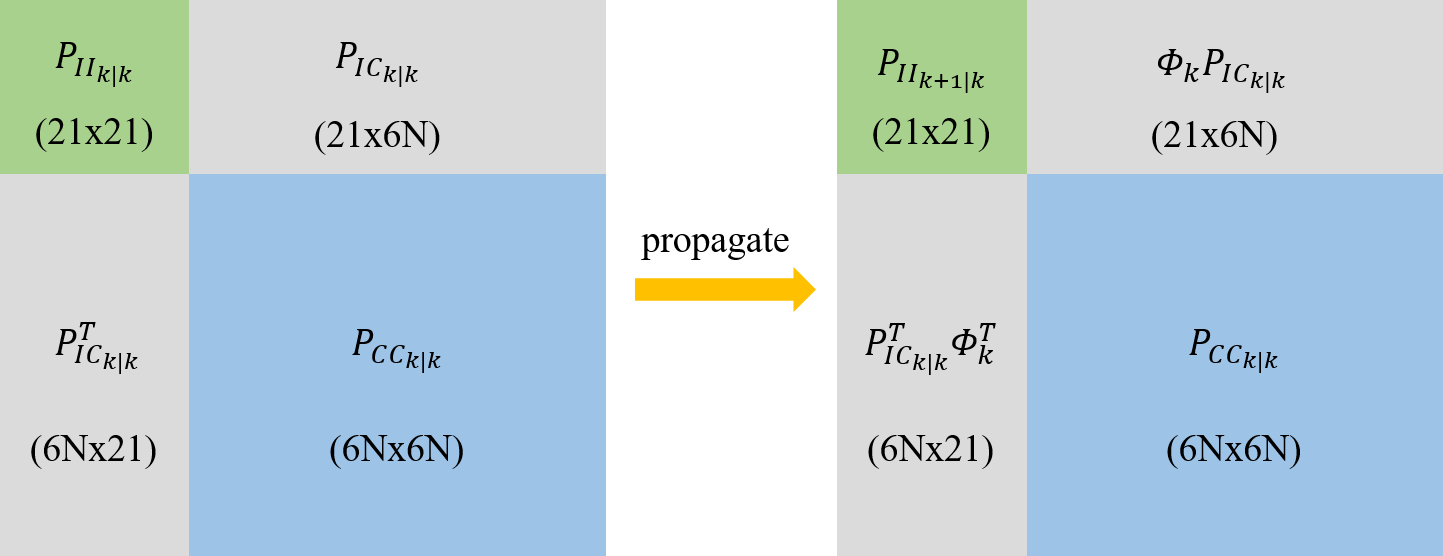
\includegraphics[scale=0.4]{images/imu_propagate.png}
\end{figure}

\subsection{State Augmentation}

代码在 \verb|MsckfVio::stateAugmentation|。

\subsubsection{相机状态向量扩增}

根据IMU位姿求取Camera位姿

\begin{equation}
\begin{aligned}
{}^C_G\hat{\mathbf{q}} = {}^C_I\hat{\mathbf{q}} \otimes {}^I_G\hat{\mathbf{q}}, \quad
{}^G\hat{\mathbf{p}}_C = {}^G\hat{\mathbf{p}}_I + C\left({}^I_G\hat{\mathbf{q}}\right)^\top {}^I\hat{\mathbf{p}}_C
\end{aligned}
\end{equation}

\subsubsection{状态协方差扩增}

增广的状态协方差矩阵为({\color{red}why})

\begin{equation}
\begin{aligned}
\mathbf{P}_{k|k}^{\prime}
= 
\begin{pmatrix}
\mathbf{I}_{21+6N} \\ \mathbf{J}
\end{pmatrix}
\mathbf{P}_{k|k}
\begin{pmatrix}
\mathbf{I}_{21+6N} \\ \mathbf{J}
\end{pmatrix}^\top 
=
\begin{bmatrix}
\mathbf{P}_{k|k} & (\mathbf{J} \mathbf{P}_{k|k})^T \\
\mathbf{J} \mathbf{P}_{k|k} & \mathbf{J} \mathbf{P}_{k|k} \mathbf{J}^T
\end{bmatrix}
\end{aligned}
\in \mathbb{R}^{(21+6N+6) \times (21+6N+6)}
\end{equation}

其中(下式参考\citep{sun2018robust},而代码参考\cite{mourikis2007multi},{\color{red}哪一个正确}),

\begin{equation*}
\mathbf{J} = 
\frac{\partial{\tilde{\mathbf{x}}_{C_i}}}{\partial{\tilde{\mathbf{x}}}} = 
\frac{
\partial{\left(
{}^{C_i}_G\tilde{\boldsymbol{\theta}}^\top \quad
{}^G\tilde{\mathbf{p}}_{C_i}^\top
\right)^\top}}
{\partial{\left(
\tilde{\mathbf{x}}_I^\top \quad
\tilde{\mathbf{x}}_{C_1}^\top \quad
\cdots \quad 
\tilde{\mathbf{x}}_{C_N}^\top
\right)^\top}} = 
\begin{pmatrix}
\mathbf{J}_I & \mathbf{0}_{6\times 6N}
\end{pmatrix}
\in \mathbb{R}^{6 \times (21+6N)}
\end{equation*}

\begin{equation*}
\mathbf{J}_I = 
\frac{\partial{\tilde{\mathbf{x}}_{C_i}}}{\partial{\tilde{\mathbf{x}}_I}} = 
\begin{pmatrix}
C\left({}^I_G\hat{\mathbf{q}}\right) & \mathbf{0}_{3\times 9} & 
\mathbf{0}_{3\times 3} & \mathbf{I}_3 & \mathbf{0}_{3\times 3} \\
-C\left({}^I_G\hat{\mathbf{q}}\right)^\top \lfloor{}^I\hat{\mathbf{p}}_C {}_{\times}\rfloor & 
\mathbf{0}_{3\times 9} & \mathbf{I}_3 & \mathbf{0}_{3\times 3} & 
\mathbf{I}_{3}
\end{pmatrix}
\in \mathbb{R}^{6 \times 21}
\end{equation*}

为表示方便,拆解 $\mathbf{P}_{k|k}$为

\begin{equation}
\mathbf{P}_{k|k} =
\begin{bmatrix}
\mathbf{P}_{11} & \mathbf{P}_{12} \\
\mathbf{P}_{21} & \mathbf{P}_{22} \\
\end{bmatrix}
\end{equation}

则

\begin{equation}
{\color{blue}
\mathbf{P}_{k|k}^{\prime} =
\begin{bmatrix}
\mathbf{P}_{k|k} & \mathbf{J}_P^T \\
\mathbf{J}_P & \mathbf{J}_I \mathbf{P}_{11} \mathbf{J}_I^T
\end{bmatrix}
\quad \text{where} \quad
\mathbf{J}_P = \left(\mathbf{J}_I \mathbf{P}_{11} \quad \mathbf{J}_I \mathbf{P}_{12}\right)
}
\end{equation}

\begin{figure}[!htbp]
\centering
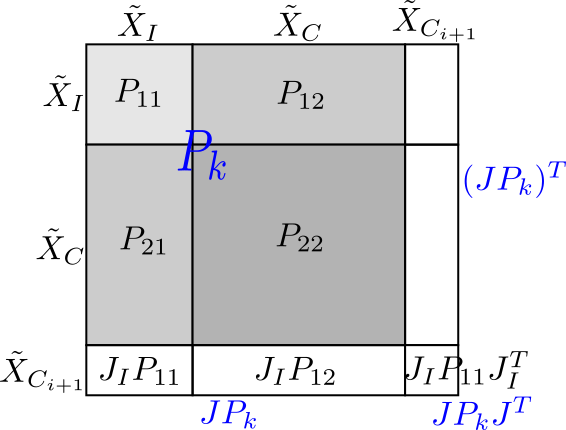
\includegraphics[scale=0.45]{images/visual_conv_augmentation.png}
\end{figure}

{\color{red}why: Fix the covariance to be symmetric}

\begin{equation}
\mathbf{P}_{k|k}^{\prime} = 
\frac{\mathbf{P}_{k|k}^{\prime} + {\mathbf{P}_{k|k}^{\prime}}^{\top}}{2}
\end{equation}


\subsection{Measurement Update}

\subsubsection{Measurement Model}

\begin{enumerate}

\item 计算获取世界坐标系下的3D特征点,代码在 \verb|Feature::initializePosition|

\begin{itemize}
\item 据对极几何原理,三角化计算初始深度,得到初始三维点坐标
\item 通过L-M算法迭代优化得到更加精确的世界系三维点
\end{itemize}

\item 投影世界系三维点到相机系

\begin{equation*}
\begin{gathered}
{}^{C_{i, 1}}\mathbf{p}_j = 
\begin{pmatrix}
{}^{C_{i, 1}}X_j \\ {}^{C_{i, 1}}Y_j \\ {}^{C_{i, 1}}Z_j
\end{pmatrix} = 
C\left({}^{C_{i, 1}}_G\mathbf{q}\right)
\left({}^G\mathbf{p}_j-{}^G\mathbf{p}_{C_{i, 1}}\right) \\
\begin{aligned}
{}^{C_{i, 2}}\mathbf{p}_j &= 
\begin{pmatrix}
{}^{C_{i, 2}}X_j \\ {}^{C_{i, 2}}Y_j \\ {}^{C_{i, 2}}Z_j
\end{pmatrix} = 
C\left({}^{C_{i, 2}}_G\mathbf{q}\right)
\left({}^G\mathbf{p}_j-{}^G\mathbf{p}_{C_{i, 2}}\right) \\
&= C\left({}^{C_{i, 2}}_{C_{i, 1}}\mathbf{q}\right)
\left({}^{C_{i, 1}}\mathbf{p}_j - 
{}^{C_{i, 1}}\mathbf{p}_{C_{i, 2}}\right)
\end{aligned}
\end{gathered}
\end{equation*} 

\item 线性化测量模型,视觉测量残差可近似表示为

\begin{equation}
\mathbf{r}^j_i = 
\mathbf{z}_i^j - \hat{\mathbf{z}}_i^j = 
\mathbf{H}_{C_i}^j\tilde{\mathbf{x}}_{C_i} + 
\mathbf{H}_{f_i}^j{}^G\tilde{\mathbf{p}}_{j} + 
\mathbf{n}_i^j
\in \mathbb{R}^{4 \times 1}
\end{equation}

其中,测量雅克比矩阵(代码在 \verb|MsckfVio::measurementJacobian|)

\begin{equation}
\begin{gathered}
\mathbf{H}_{C_i}^j = 
\frac{\partial \mathbf{z}_i^j}{\partial {}^{C_{i,1}}\mathbf{p}_j} \cdot 
\frac{\partial {}^{C_{i,1}}\mathbf{p}_j}{\partial \mathbf{x}_{C_{i,1}}} + 
\frac{\partial \mathbf{z}_i^j}{\partial {}^{C_{i,2}}\mathbf{p}_j} \cdot 
\frac{\partial {}^{C_{i,2}}\mathbf{p}_j}{\partial \mathbf{x}_{C_{i,1}}}
\in \mathbb{R}^{4 \times 6} \\
\mathbf{H}_{f_i}^j = 
\frac{\partial \mathbf{z}_i^j}{\partial {}^{C_{i,1}}\mathbf{p}_j} \cdot 
\frac{\partial {}^{C_{i,1}}\mathbf{p}_j}{\partial {}^G\mathbf{p}_j} +
\frac{\partial \mathbf{z}_i^j}{\partial {}^{C_{i,2}}\mathbf{p}_j} \cdot 
\frac{\partial {}^{C_{i,2}}\mathbf{p}_j}{\partial {}^G\mathbf{p}_j} 
\in \mathbb{R}^{4 \times 3}
\end{gathered}
\end{equation}

{\color{red}{why: Modifty the measurement Jacobian to ensure observability constrain, Ref: OC-VINS}}

\item 叠加对同一特征点的多个观测(代码在 \verb|MsckfVio::featureJacobian|)

\begin{equation*}
\mathbf{r}^j = 
\mathbf{H}_{\mathbf{x}}^j \tilde{\mathbf{x}} + 
\mathbf{H}_f^j {}^G\tilde{\mathbf{p}}_j + 
\mathbf{n}^j
\quad \text{with} \quad
\mathbf{H}_{\mathbf{x}}^j \in \mathbb{R}^{4M \times 6}, 
\mathbf{H}_f^j \in \mathbb{R}^{4M \times 3}
\end{equation*}

为避免${}^G\mathbf{p}_j$的不确定性对测量残差的影响,将残差投影到$\mathbf{H}_{f_i}^j$的左零空间 $\mathbf{V} \in \mathbb{R}^{4M \times (4M-3)}$

\begin{equation}
\mathbf{r}^j_o 
= \mathbf{V}^\top \mathbf{r}^j
= \mathbf{V}^\top \mathbf{H}_{\mathbf{x}}^j\tilde{\mathbf{x}} +
\mathbf{V}^\top \mathbf{n}^j
= \mathbf{H}_{\mathbf{x}, o}^j\tilde{\mathbf{x}} + 
\mathbf{n}^j_o 
\in \mathbb{R}^{(4M-3) \times 1}
\end{equation}

零空间$\mathbf{V}$通过SVD分解得到(代码在 \verb|MsckfVio::featureJacobian|)
\begin{lstlisting}
// Project the residual and Jacobians onto the nullspace of H_fj.
JacobiSVD<MatrixXd> svd_helper(H_fj, ComputeFullU | ComputeThinV);
MatrixXd A = svd_helper.matrixU().rightCols(jacobian_row_size - 3);
H_x = A.transpose() * H_xj;
r   = A.transpose() * r_j;
\end{lstlisting}

\item 叠加所有特征点的多个观测,得到

\begin{equation}
\label{equ:visual_residual_final}
\mathbf{r}_{o}=\mathbf{H}_{\mathbf{X}} \widetilde{\mathbf{X}}+\mathbf{n}_{o}
\in \mathbb{R}^{N(4M-3) \times 1}
\end{equation}

\begin{lstlisting}
if (gatingTest(H_xj, r_j, cam_state_ids.size()-1)) {
  H_x.block(stack_cntr, 0, H_xj.rows(), H_xj.cols()) = H_xj;
  r.segment(stack_cntr, r_j.rows()) = r_j;
  stack_cntr += H_xj.rows();
}
\end{lstlisting}

\end{enumerate}


\subsubsection{能观性约束}

OC-EKF


\subsubsection{EKF Update}

代码在 \verb|MsckfVio::measurementUpdate|。

根据~\cite{mourikis2007multi},为降低EKF更新的计算复杂度,对$\mathbf{H}_{\mathbf{X}}$进行QR分解

\begin{equation}
\mathbf{H}_{\mathbf{X}}=\left[\begin{array}{ll}{\mathbf{Q}_{1}} & {\mathbf{Q}_{2}}\end{array}\right]\left[\begin{array}{c}{\mathbf{T}_{H}} \\ {\mathbf{0}}\end{array}\right]
\end{equation}

带入式~\eqref{equ:visual_residual_final},得

\begin{equation}
\mathbf{r}_{o}=\left[\begin{array}{ll}{\mathbf{Q}_{1}} & {\mathbf{Q}_{2}}\end{array}\right]\left[\begin{array}{c}{\mathbf{T}_{H}} \\ {\mathbf{0}}\end{array}\right] \tilde{\mathbf{X}}+\mathbf{n}_{o}
\end{equation}

\begin{equation}
\left[\begin{array}{l}
{\mathbf{Q}_{1}^{T} \mathbf{r}_{o}} \\ {\mathbf{Q}_{2}^{T} \mathbf{r}_{o}}\end{array}\right]=\left[\begin{array}{c}{\mathbf{T}_{H}} \\ {\mathbf{0}}\end{array}\right] \tilde{\mathbf{X}}+\left[\begin{array}{l}{\mathbf{Q}_{1}^{T} \mathbf{n}_{o}} \\ {\mathbf{Q}_{2}^{T} \mathbf{n}_{o}}\end{array}\right]
\end{equation}

上式${\mathbf{Q}_{2}^{T} \mathbf{r}_{o}}$仅含有噪声,对其忽略,取$\mathbf{Q}_{1}^{T} \mathbf{r}_{o}$用于EKF更新

\begin{equation}
\mathbf{r}_{n}=\mathbf{Q}_{1}^{T} \mathbf{r}_{o}=\mathbf{T}_{H} \widetilde{\mathbf{X}}+\mathbf{n}_{n}
\end{equation}

噪声向量$\mathbf{n}_{n}$的协方差矩阵为

\begin{equation}
\mathbf{R}_{n}=
\mathbf{Q}_{1}^{T} \mathbf{R}_{o} \mathbf{Q}_{1}=\sigma_{\mathrm{im}}^{2} \mathbf{I}_{r}
\end{equation}

计算Kalman增益

\begin{equation}
\mathbf{K}=\mathbf{P} \mathbf{T}_{H}^{T}\left(\mathbf{T}_{H} \mathbf{P} \mathbf{T}_{H}^{T}+\mathbf{R}_{n}\right)^{-1}
\end{equation}

更新系统误差状态

\begin{equation}
\Delta \mathbf{X}=\mathbf{K r}_{n}
\end{equation}

更新系统状态

\begin{equation}
\mathbf{X}_{k+1} = \mathbf{X}_k \oplus \Delta \mathbf{X}
\end{equation}

更新系统状态协方差矩阵

\begin{equation}
\mathbf{P}_{k+1 | k+1}=\left(\mathbf{I}_{\xi}-\mathbf{K} \mathbf{T}_{H}\right) \mathbf{P}_{k+1 | k}\left(\mathbf{I}_{\xi}-\mathbf{K} \mathbf{T}_{H}\right)^{T}+\mathbf{K} \mathbf{R}_{n} \mathbf{K}^{T}
\end{equation}

\newpage

\bibliography{bibfile}

\end{document}